\documentclass[11pt,a4paper,titlepage]{report}

\usepackage[utf8]{inputenc}
\usepackage[english]{babel}
\usepackage{csquotes}

\usepackage{listings}
\usepackage{xcolor}
\usepackage[none]{hyphenat}
\usepackage{textcomp}
\usepackage{parskip}

\usepackage{graphicx}
\graphicspath{ {images/} }

\author{Cyrus Hanlon}
\title{A Scriptable 2D Game Engine}

%Library
\usepackage[backend=bibtex,style=numeric]{biblatex}
\addbibresource{document.bib}

\setlength{\parskip}{1em}

\begin{document}
	\maketitle
	
	\definecolor{listinggray}{gray}{0.9}
	\definecolor{lbcolor}{rgb}{0.95,0.95,0.95}
	\lstdefinestyle{C++}{
		language=[GNU]C++,
		backgroundcolor=\color{lbcolor},
		captionpos=b,
		tabsize=4,    
		%   rulecolor=,
		basicstyle=\footnotesize,
		upquote=true,
		aboveskip={1.5\baselineskip},
		columns=fixed,
		showstringspaces=false,
		extendedchars=false,
		breaklines=true,
		numbersep=5pt,
		prebreak = \raisebox{0ex}[0ex][0ex]{\ensuremath{\hookleftarrow}},
		frame=lines,
		numbers=left,
		showtabs=false,
		showspaces=false,
		showstringspaces=false,
		identifierstyle=\ttfamily,
		keywordstyle=\color[rgb]{0,0,1},
		commentstyle=\color[rgb]{0,0.392,0},
		stringstyle=\color{red},
		numberstyle=\color[rgb]{0.205, 0.142, 0.73},
	}
	\lstdefinestyle{Lua}{
		language=[5.2]Lua,
		backgroundcolor=\color{lbcolor},
		captionpos=b,
		tabsize=4,    
		%   rulecolor=,
		basicstyle=\footnotesize,
		upquote=true,
		aboveskip={1.5\baselineskip},
		columns=fixed,
		showstringspaces=false,
		extendedchars=false,
		breaklines=true,
		numbersep=5pt,
		prebreak = \raisebox{0ex}[0ex][0ex]{\ensuremath{\hookleftarrow}},
		frame=lines,
		numbers=left,
		showtabs=false,
		showspaces=false,
		showstringspaces=false,
		identifierstyle=\ttfamily,
		keywordstyle=\color[rgb]{0,0,1},
		commentstyle=\color[rgb]{0,0.392,0},
		stringstyle=\color{red},
		numberstyle=\color[rgb]{0.205, 0.142, 0.73},
	}

	\tableofcontents{}
	\newpage

\chapter{Introduction}
		
%A statement of the aims of the work and a brief overview of the remainder of the report.

	There are many game engines that already exist but nothing combines ease of use with raw speed.
	
	From Unreal Engine~\cite{UE} with its complete design versus much lighter weight engines such as LÖVE~\cite{LOVE}, there is a very wide range of technologies and techniques at work. There is a definitive gap between large heavy engines and the small and lightweight that I intend to fill. By having many features written into the core engine but keeping a lightweight and easy to use API at the front, it will be possible to quickly learn how to prototype games, as well as, achieve excellent real world performance.

	A very important part of any game engine is the interface between developer and the inner workings. There are many scripting languages that can be chosen from and there are many important factors when selecting a language to use, the most important factors include: popularity, execution speed and learning curve. Lua is at the top of the pile when it comes to games. Other languages such as JavaScript and Python are extremely popular in other areas but are not anywhere near as often used in games as they are more difficult to bind.
				
	Embedded scripting languages need to have access to core elements of the game engine to allow for developers to create fully fledged games without having to touch the lower level. Having the core engine open source also allows game developers to extend the Lua interface as required and push the changes to the repository.

	Over the course of this report the design, implementation and technologies involved will be discussed including library choice for the various aspects as required.
	
\newpage










	
\chapter{Literature Review}

%Relate your work to previous work (literature). Give the context of the Analysis work and any technical details necessary for understanding the work. Establish motivation for the present work.

\section{Lua}
\subsection{About Lua}
	Lua was created for extending applications, there was an increase in demand for customisation and no was language available that combined procedural features with powerful data description facilities.~\cite{Ierusalimschy02software} Lua came from the languages SOL and DEL~\cite{Ierusalimschy01theevolution} both of which were made by the company Tecgraf.
	
	SOL is an acronym for Simple Object Language was a specialized data description language used for customising software. The SOL syntax was strongly influenced by the syntax of BiBTeX~\cite{Lamport:1989:LDP:63364}. DEL is an acronym for Data Entry Language, an entity in DEL is essentially an object or record in other languages~\cite{Ierusalimschy01theevolution}. Lua was created as a unique combination of the two more primitive languages, it was designed to avoid unique syntax so that anyone could use it effectively with limited training and for the language to have built in type checking.
	
	Lua is written in C and so, is very cross platform~\cite{LuaSource}, it is used in projects ranging from Cheat Engine~\cite{CheatEngine}, an open source memory scanner and hex editor for Windows, to Android and iOS games using something such as Cocos2d~\cite{COCOS2D}, an open source software framework used in the creation of apps or games. Therefore Lua is widely used thanks to its simple learning curve, ease of implementation using the provided minimalistic C API and its fast execution when compared to similar languages. It is also used in many non game settings such as in embedded systems using eLua~\cite{eLua} thanks to its low memory footprint.

	Lua allows for loading modules at run time that were not required at build time, this allows for extremely flexible program extensions. A module is made available through the use of an ordinary table with functions or variables being accessed through the table. Loading, compiling then executing Lua files from within Lua is easily possible and allows for things such as hot reloading code vastly improving the development rate as developers could just save a file and the Lua program would simply start using it.
		
\subsection{Running Lua}
	Lua is not interpreted directly but is instead compiled into bytecode, this is then run on the Lua virtual machine. Because of this Lua is a fast language, considering how high level it is. Lua used a stack based virtual machine initially but with the release of Lua 5.0, Lua began to use a register based machine. It also uses a stack for allocating activation records where the registers live~\cite{IerusalimschyImplementation}.

	First class functions with lexical scoping is difficult to implement for languages that use a stack based vm, Lua uses a stack for local variables and a heap for when they go out of scope while being referenced to by nested functions~\cite{IerusalimschyImplementation}. Using this concept Lua successfully implements features such as closures that rely on register based VMs.

	Lua can also be used from the command line which allows for productivity scripts to be written and used without the need for it to be embedded into another application. Lua can also be used as a standalone program using the tool srLua which was created by one of the Lua authors~\cite{tecgrafLibAndTools}, this allows the language to be used almost anywhere on almost anything.

\subsection{Syntax}
	The syntax of Lua was designed so that it combined simple procedural syntax with powerful data description constructs, the general syntax is very easy to learn with its roots in SOL and DEL, both were designed for ease of use. It borrows much of its syntax from other languages, its comment syntax, for example, is similar to that of Haskell and SQL. It's control flow is similar to that of pascal using keywords such as \texttt{then} and \texttt{end} for \texttt{if} statements. It is, however, renowned for being very easy to write with its simple syntax and extremely powerful table constructs. A quirk when working with Lua is the fact that tables start at an index of 1 instead of 0 as is very common throughout programming languages.

	An example of Lua's control statements are shown in listing~\ref{lst:SyntaxSample1}. The use of \texttt{elseif} as a single keyword is useful and avoids the need to use an \texttt{end} per \texttt{if}. The conditions in each of the statements do not need to be wrapped in parenthesis and allow for logical operators. 

	\lstinputlisting[style=Lua, label={lst:SyntaxSample1}, caption={Lua Syntax Sample 1}, firstline=63, lastline=80]{codeSamples/1.lua}

	There are two types of \texttt{for} loop in Lua, one is a numeric \texttt{for} and is shown in listing~\ref{lst:SyntaxSample1}, the other is the generic \texttt{for} that uses an iterator and allows for the traversal of all values. The numeric \texttt{for} uses a very simple syntax and so is very easy to write, the first argument is the starting value of the iteration variable, the second is the end value and the third is the value to add with each loop.

	The logical operators in Lua are \texttt{and}, \texttt{or} and \texttt{not}. Logical operators and control statement expressions take \texttt{nil} and \texttt{false} as \texttt{false} and anything else as \texttt{true}~\cite{LuaMan} This allows for some unique syntax that more advanced Lua programmers will use to reduce the amount of code required.

	Each of the three logical operators behave differently when used in this way. The \texttt{and} operator returns its first argument if it is \texttt{false} and otherwise returns its second argument. The \texttt{or} operator returns its first argument if this value isn't \texttt{false} and returns its second argument otherwise. The \texttt{not} operator always returns \texttt{true} or \texttt{false} based on the argument. The Lua 5.3 manual~\cite{LuaMan} has an excellent set of examples as shown in listing~\ref{lst:SyntaxSample2}.
	\lstinputlisting[style=Lua, label={lst:SyntaxSample2}, caption={Lua Syntax Sample 2 (taken from \cite{LuaMan})}, firstline=82, lastline=89]{codeSamples/1.lua}

	Using this behaviour of logical operators allows for quickly and easily assigning variables using, for example, a configuration file.

	Lua allows for assigning multiple variables on the same line as shown in listing~\ref{lst:SyntaxSample3}. When used in conjunction with returning multiple values from a function this can reduce the amount of code required and therefore improve development time.
	\lstinputlisting[style=Lua, label={lst:SyntaxSample3}, caption={Lua Syntax Sample 3}, firstline=134, lastline=135]{codeSamples/1.lua} 

	With the introduction of Lua 5.2, the \texttt{bit32} library added support for bitwise operations and with Lua 5.3 came native support for bitwise operators. Behaviour is exactly the same as in any other language with support for them as is shown in listing~\ref{lst:bitwise1}.
	\lstinputlisting[style=Lua, label={lst:bitwise1}, caption={Lua Bitwise Operations}, firstline=137, lastline=142]{codeSamples/1.lua} 

	Lua has some syntactic sugar which helps to simplify what the Lua developer will have to interact with.
	
	\lstinputlisting[style=Lua, label={lst:SyntacticSugarSample1}, caption={Syntactic Sugar Sample 1}, firstline=1, lastline=8]{codeSamples/1.lua}
	In listing~\ref{lst:SyntacticSugarSample1} we can see how to inline declare a table with a sub table that is also inline declared.

	\lstinputlisting[style=Lua, label={lst:SyntacticSugarSample2}, caption={Syntactic Sugar Sample 2}, firstline=17, lastline=21]{codeSamples/1.lua}
	We can see how to declare a member function using some syntactic sugar in listing~\ref{lst:SyntacticSugarSample2}. Which is equivalent to listing~\ref{lst:SyntacticSugarSample3}.

	\lstinputlisting[style=Lua, label={lst:SyntacticSugarSample3}, caption={Syntactic Sugar Sample 3}, firstline=10, lastline=15]{codeSamples/1.lua}

	There are also several ways to access entries within a table all of which can be mixed and matched based on the programmers preference.

	\lstinputlisting[style=Lua, label={lst:SyntacticSugarSample4}, caption={Syntactic Sugar Sample 4}, firstline=23, lastline=25]{codeSamples/1.lua}

	Lua's support for coercion allows for the automatic conversion of strings and numbers, this helps developers with rapid development as they would not need to have to think about converting types in many situations when Lua itself handles it for them. Bitwise operators always convert numbers to integers, mathematic operations always convert operands to floats ~\cite{LuaMan}.
	
	String concatenation using the \texttt{..} operator converts numbers to strings wherever is needed but using the \texttt{string.format} function will allow for fine tuned control of how the number will be converted.

	Examples of Lua's coercion in action are shown in listing~\ref{lst:Coercion 1}.
	\lstinputlisting[style=Lua, label={lst:Coercion 1}, caption={Coercion Sample 1}, firstline=144, lastline=148]{codeSamples/1.lua}

	Lua's tables have a length operator in the form of \texttt{\#}, it returns the length of a table as would be found by the \texttt{ipairs} operator. It counts through integers starting at 1 and stopping when the first nil value is found, this means that the operator is only useful for finding the length of array-like tables.

\subsection{Functions}
	Lua allows for a function to return multiple values, this is an interesting concept and can have some downsides, it can make it quite difficult to correctly name a function to reflect the return values. It is a very powerful feature and if handled correctly can improve productivity especially when combined with Lua's variable number of arguments. An example is shown in listing~\ref{lst:Functions1}.
	\lstinputlisting[style=Lua, label={lst:Functions1}, caption={Functions Sample 1}, firstline=97, lastline=105]{codeSamples/1.lua}

	Functions, in Lua, are first class values with proper lexical scoping~\cite{Ierusalimschy:2013:PLT:2502646}. A first class value in Lua means that a function is essentially the same as any other regular variable, this allows a Lua developer to pass functions into other functions as arguments, return functions, use functions of keys and values of tables and can be assigned to a variable. This is a very valuable trait for a high level scripting language to have as it allows for very interesting techniques such as functional programming, closures are fully supported in Lua as a result of this.

	Lua has proper tail calls which allows for recursion. If the last thing that a function does is call another function, the calling function is no longer required and is no longer required on the stack, this allows for an infinite recursion without overflowing the stack~\cite{Ierusalimschy:2013:PLT:2502646}. An example of a Lua tail call is shown in listing~\ref{lst:Functions2}.
	\lstinputlisting[style=Lua, label={lst:Functions2}, caption={Functions Sample 2}, firstline=91, lastline=95]{codeSamples/1.lua}

	Without proper tail calls, recursion could overflow the stack but with proper tail calls this is impossible and fits in perfectly with a high level scripting language such as Lua.

\subsection{Tables}
	Tables are the only data structure in Lua but are extremely flexible and can be used to provide the functionality of almost any data structure as required. They are very similar in use to a hash map and allow for any variable of any type to be assigned to a key or value within the same table with the exception of \texttt{nil}, it is also possible to treat a table similar to an array as shown in listing~\ref{lst:TablesSample1}.
	\lstinputlisting[style=Lua, label={lst:TablesSample1}, caption={Tables in Lua Sample 1}, firstline=27, lastline=36]{codeSamples/1.lua}

	Lua has a variety of built in functions for the use of manipulating and getting data from tables all available through the table library~\cite{LuaMan}.

	To loop over all key-value pairs in a table lua provides the \texttt{ipairs} and \texttt{pairs} iterators. Used with a \texttt{for} loop a Lua developer is provided with a powerful method of quickly and easily accessing anything within a table as shown in listing~\ref{lst:TablesSample2}.
	\lstinputlisting[style=Lua, label={lst:TablesSample2}, caption={Tables in Lua Sample 2}, firstline=38, lastline=61]{codeSamples/1.lua}

	The \texttt{pairs} function iterates over all elements in a table while the \texttt{ipairs} function will return all key-value pairs where the keys are numbers, starting at the first index and stopping when it hits the first nil value.~\cite{Ierusalimschy:2013:PLT:2502646} 
	
	Getting the length of a Lua array is found by calling \texttt{table.getn(tab)} however, to find the size of a table with mixed key types or non-consecutive indices, a generic \texttt{for} loop with a count variable would have to be used. In cases where mixed key types are used it shouldn't be required to know the size as the pairs cannot be accessed by a normal for loop in any case.

	Weak tables are tables that consist of elements that are weak references, this can be the keys or the values, if the only reference left to an object is a weak reference the garbage collector collects it. They are often used when a word needs to be reserved without actually creating an object in memory.
	
\subsection{Metatables and Object Oriented Programming}
	All tables in Lua are permitted to have a metatable\cite{Ierusalimschy:2013:PLT:2502646}. They allow for changing the behaviour of various aspects of a lua table, such as the add operator, by setting the \texttt{\_\_add} value to a new function this code will be called instead of the default add functionality as is shown in listing~\ref{lst:MetaTables1}.
	\lstinputlisting[style=Lua, label={lst:MetaTables1}, caption={Metatables Sample 1}, firstline=107, lastline=117]{codeSamples/1.lua}

	These functions are called metamethods and allow for any interaction with a table to be altered. While classes do not exist in Lua, using a meta table and first class value functions, behaviour similar to object oriented programming can be achieved especially with the use of factory methods. An example of a class is shown in listing~\ref{lst:MetaTables2}. On line 13 a table with the metatable \texttt{Dog} is created and returned to \texttt{myDog}.
	\lstinputlisting[style=Lua, label={lst:MetaTables2}, caption={Metatables Sample 2}, firstline=119, lastline=132]{codeSamples/1.lua}

	While this concept is very useful, if the \texttt{new} function is ever changed by mistake, a difficult to locate bug could be created.

\subsection{Couroutines}
	A coroutine is similar to a thread in that it has its own line of execution, its own stack, its own local variables, and its own instruction pointer but shares global variables and almost anything else with other coroutines. The main difference to a thread is that a program with threads runs things concurrently while a coroutine in Lua is collaborative and at any given time only 1 is running~\cite{Ierusalimschy:2013:PLT:2502646}. While there may not be a performance gain from using coroutines, it allows a developer to easily orchestrate multitasking that would otherwise be difficult to implement.

	To create a coroutine it is as simple as calling the \texttt{coroutine.create} and passing a function as shown in listing~\ref{lst:Couroutine1}.
	\lstinputlisting[style=Lua, label={lst:Couroutine1}, caption={Couroutine Sample ~\cite{Ierusalimschy:2013:PLT:2502646}}, firstline=150, lastline=153]{codeSamples/1.lua} 

\subsection{Garbage Collection}

	Lua automatically manages memory, Lua destroys objects when all references to them are lost. There is no function to delete them manually, a program can only create objects which means that the developer will not need to bother with the majority of memory management~\cite{Ierusalimschy:2013:PLT:2502646}. Lua has no issues dealing with cyclic references unlike simple garbage collectors. Lua allows for manually calling the garbage collector using the \texttt{collectgarbage} function as even the best garbage collector isn't perfect, the Lua garbage collector sometimes needs some help. It is even possible to manually pause, stop and restart the garbage collector to allow for fine tuned adjustments to the use of memory in a Lua program, it is also possible to get the total amount of memory being used.

	In very high performance scenarios a Lua developer may need to assume control of the garbage collector, a simple example is shown in listing~\ref{lst:GC1}.
	\lstinputlisting[style=Lua, label={lst:GC1}, caption={Manual Garbage Collector Sample}, firstline=155, lastline=165]{codeSamples/1.lua}
	
	Although the reference to the table is removed the table still exists in memory until the next pass of the garbage collector.

\subsection{The Lua C API}

	Lua is an embedded extension library and cannot be used as a stand alone program, a program can use Lua with little input from a programmer using the provided C API. The API puts flexibility and simplicity above all else, this can sometimes make it difficult to implement for an inexperienced C developer as there is no built in type checking and no clean errors, this is down to the developer to handle ~\cite{Ierusalimschy:2013:PLT:2502646}.

	A major component of the Lua C API is that new functions can be registered with the virtual machine allowing for behaviour that would be otherwise impossible to implement in pure Lua. Class like objects called userdata can also be implemented in C and used in Lua allowing for interaction between the program and Lua, in the case of a game engine, objects such as sprites could be accessed in both C and Lua and provide a developer with the ability to create high performance games in a much easier to use package than C.

	An example of registering a function in the Lua vm is shown in listing~\ref{lst:CAPISample1}.
	\lstinputlisting[style=Lua, label={lst:CAPISample1}, caption={Sample function implementation in C API~\cite{Ierusalimschy:2013:PLT:2502646}}, firstline=1, lastline=12]{codeSamples/1.cpp}

\newpage

\section{Game Engines}
	
	There are many game engines already out there covering a wide range of performance and development styles, engines such as Unreal Engine~\cite{UE} and Unity~\cite{Unity} have integrated development environments and require all development to be done through them. Other game engines, such as LÖVE~\cite{LOVE} can be developed in any text editor using any work flow that the developer chooses, this improves prototyping times and allows developers to get comfortable much quicker as they are using tools that they are well used to.

	Open source allows for the collaborative development of any project and would therefore be ideal for a game engine, by allowing people to fork and extend a game engine a very wide variety of features can be implemented, enabled and disabled based on the individuals needs.

\subsection{LÖVE}
	LÖVE~\cite{LOVE} provides a limited set of features and leaves the majority of the work on the internals of the engine to the game developer. This allows for very fast prototyping of small example games but when creating a larger game things can get difficult. The engine does include some things at a lower level such as physics, GLSL shaders, image loading, TCP and UDP networking. Because LÖVE doesn't manage entities there is quite a low performance ceiling especially with the addition of lighting and particles, other engines address this at the cost of development time. LÖVE is completely open source and completely free.
\subsection{Unity and Unreal Engine}
	Unity~\cite{Unity} and Unreal Engine~\cite{UE} both manage every aspect of the game while still allowing massive extensibility. Both have unique development flows and both take a very long time to master, because of just have massive they are, development can be very slow when compared to lightweight prototyping engines. The Unity engine is not fully open source but allows source access for certain modules of the engine while the latest versions of Unreal Engine are fully open source, both adopt similar payment patterns making the developer pay based on the number of sales rather than a fixed fee, this allows for smaller studios and individuals to create very professional games.
\subsection{Cocos2d}
	Cocos2d is an open source framework designed for creating cross platform games, apps and other GUI based programs~\cite{COCOS2D}, it has support for scripting in both Lua and JavaScript but requires C++ code to initialize any scripts. There is an IDE created for cocos2D that provides similar workflow to the full engines while having the flexibility of text only engines such as LÖVE.










\chapter{Design}

%State the identified requirements and show design diagrams with full explanations for your product.

%The main goal is that students use this progress report to schedule their work and allow supervisors an opportunity to comment on the approach taken by students and the level of progress made.

	Using an agile methodology will be an important part of the development of this project as it provides a far superior work flow as opposed to far more static methodologies such as the waterfall method. This will result in an improved rate of work and the addition of currently undiscovered ideas.

%Write about requirements

	For a game engine to be a complete engine a wide variety of features are required especially when a high level scripting language is the only input for developers to use when creating a game.

	The engine will provide a Lua interface to all required core engine features using the Lua C API.

	The engine will need the ability to render, reposition, angle and animate sprites provided from a spritesheet.

	Physics will also need to be provided by the engine to allow for much improved performance over having physics implemented in Lua.

	Both the physics and rendering capabilities of the game engine will need to be fully accessed through the provided Lua API. The Lua API should be consistent and easy to use, matching, where possible, the Lua style completely.

%Write about lib choices for each part

	Parts of the engine will be handled by external libraries, an important property of these libraries is performance and modernness as well as cross platform capability. Ideally the libraries will be open source.

	Rendering, physics, scripting and sound will be handled by external libraries and implemented in the game engine. For rendering and sound there are several choices: SDL, SFML, DirectX and OpenGL with a sound library. SDL is widely used and has very good performance but it is written in pure C so has no object oriented code and is therefore quite dated when compared to SFML. DirectX is only available on the windows and Xbox platforms and is therefore not ideal for this project as cross platform is a requirement. OpenGL with a sound library has the best performance of all of the options but is also the most difficult to use and both SDL and SFML wrap OpenGL and provide access to the context so would be better options.

	SFML or Simple and Fast Multimedia Library is written in C++ and is available on Linux, Mac, Windows and FreeBSD and is fully open source with its code available on github. SFML handles everything from window management and input to sound and networking, the performance is very similar to that of SDL but provides a modern object oriented API unlike SDL. These reasons make SFML the perfect choice for the projects requirements.

	For the physics library there is only one real option when it comes to games. Box2d is an open source C++ physics engine for simulating rigid bodies in 2D~\cite{Box2D}. It has excellent performance and is well proven for it's suitability for this project as many games and game engines on all platforms use it to great effect.

	As for scripting the game engine there are several options such as C\#, Javascript and Lua. For the purposes of this project, Lua is the best option due to it's simple binding process and powerful syntax. Many games use Lua as their embedded scripting language such as Garry's Mod, World of Warcraft, Angry Birds and many, many more.

%Write what needs to be done and in what order 

	The first step to creating a game engine is to get each of the libraries working correctly in a single project. As the project will be completed in an agile fashion it may be difficult to know exactly what will be created and in what order, however, that does not mean that designs can be drawn up outlining potential solutions.

	The engine will require a variety of features including an entity management system, such as the entity component system, this will allow for dynamic game objects that are easily pieced together by a developer. This system will need to manage a wide variety of entities in various forms including drawing, animating, playing sounds and others. An example entity that will behave as a player controlled car would have the following class diagram, the entity component system example is shown in \ref{fig:ClassDiagram1}.

	\begin{figure}[h] 
		\centering
		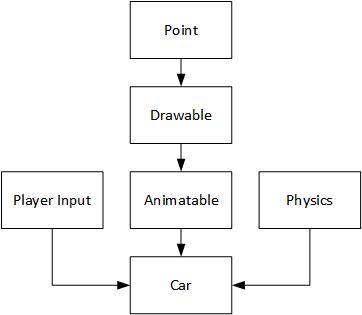
\includegraphics[scale=0.75]{ECS1}
		\caption{ECS Class Diagram Example}
		\label{fig:ClassDiagram1}
	\end{figure}

	For a car to be functional in a game it will need to be drawn and animated, have a physical presence in the world and receive player input. Behaviour can be easily placed into new components when repeated code is required, in the static inheritance system this is not as simple.

	\begin{figure}[h]
		\centering
		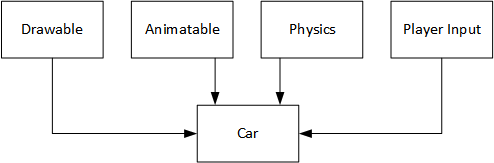
\includegraphics[scale=0.75]{ECS2}
		\caption{ECS Class Diagram Example}
		\label{fig:ClassDiagram2}
	\end{figure}

	Another example of the same in game behaviour in the more traditional class hierarchy system is much simpler to implement but doesn't allow for the dynamism of the entity component system as is shown in \ref{fig:ClassDiagram2} and the diagram is clearly more complicated and may result in repeated code. For the sake of development it may be better to first implement the more traditional system and then convert over to the ECS style.

	Lua script management will be entirely handled within the core of the game engine allowing for creating and removing objects, managing object behaviour, physics interactions, UI, the camera and more. The engine will be a completely open source and will be easily expandable and improvable by the community as a result.

	For the UI an external library created to provide UI capabilities to SFML could be used such as SFGUI or TGUI. This will need binding for use in Lua which could prove to be challenging, however getting the minimum working example would not be too difficult. It may be better for the development time if only text rendering is implemented as other UI elements can be achieved using sprites.

	Loading and saving of the game state should be integrated into the game engine to speed up development time for the game developer. Level loading should also be integrated, an external open source level editor application could be used for the creation of the levels, a json or other data file could then be loaded into the game engine reducing the development time even further. Settings should also be managed by the game allowing the Lua developer to load and save any required key value pairs using a provided API, by implementing these features in the game engine the game developer can focus more on the actual game rather than semantics.

	Documentation is a requirement for people to be able to use the engine to create games effectively and helps to reduce the learning curve. Each part of the documentation should be completed after the completion of every Lua accessible feature to ensure that it is kept on top of. Some kind of automatic documentation tool could be used similar to that of Golang's GoDoc or Java's javadoc, this would allow for the the documentation to stay up to date given any changes to the underlying code. Well documented examples could mitigate the requirement for extensive documentation, however, both would be ideal.

	%Design stuff 
	
	For the game engine to function well there are a number of required systems that must be incorporated into the core of the engine. There are 5 main elements, the window, the physics world, the resource manager, the gamestate manager and the Lua state.

	\begin{figure}[h] 
		\centering
		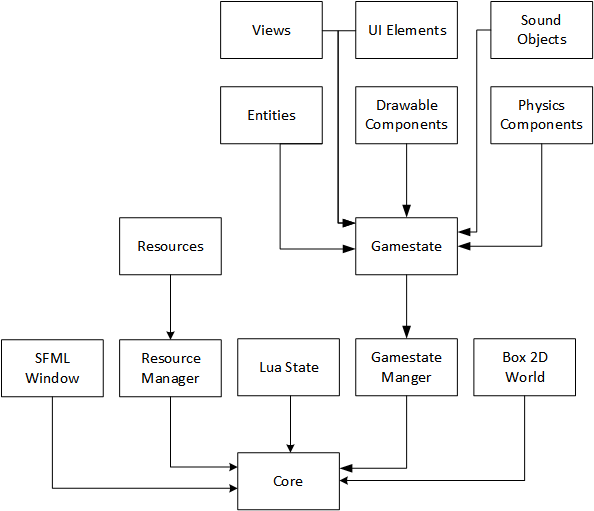
\includegraphics[scale=0.75]{core1}
		\caption{Core Systems Diagram}
		\label{fig:CoreDiagram1}
	\end{figure}

	In figure \ref{fig:CoreDiagram1} the design of the core is outlined, any lateral connections will be available to each system through the core, drawable components and sound objects will have access to the resource manager.

	%pseudo code of gamestate
	\lstinputlisting[style=Lua, label={lst:pseudo1}, caption={Gamestate Pseudo Code}, firstline=0, lastline=18]{codeSamples/pseudocode.code}

	%pseudo code/diagrams of ECS


	%resource manager pseudo


	%components










\chapter{Implementation}

	%Describe the work undertaken and the results obtained.  Small sections of code can  be  used  to  aid  the  understanding  of  a  particular  point.   Discuss  testing strategy and show testing details.

	%Got project building with Lua and SFML
    
    An important first step was to get Lua, SFML and Box2D building together within a single cpp project. Once the project was building correctly, the next step was to create some example classes and a simple main program loop to create a test bed for future work.

    At each major stage in the development cycle testing the game engine on other platforms was ensured as a cross platform game engine is far more useful to a developer than one that is locked down to a specific platform.

%Created example class in C++ that works in SFML
%Designed and created first classes of the entity system
%Created drawable and point classes
    
    Creating simple classes that showed that SFML works allowed for the creating of the first classes as shown in the class diagram. The drawable and point classes were then created as well as the surrounding framework to allow for the storing and retrieval of the objects from both Lua and in cpp tests.

    The point class is purely virtual and cannot be instantiated, it provides a think function that will be overridden by all sub classes that are required to do work every cycle of the main loop. This style of programming reduces the amount of duplicated code in the core of the engine.

    The drawable class provides the ability to draw a sprite at a set position and inherits from the point class so that it can be stored in the same vector as other entities and can then be casted as is required. This is a standard example of using the type theory of polymorphism~\cite{PolymorphismDef} and allows for all subtypes to be handled by the same functions while having, potentially, fully unique behaviour.

%Designed and created resource manager

    Creating the resource manager proved to be challenging but ultimately very satisfying when it worked correctly. It allows for the end user of the game engine to not have to bother with resource management as the core engine will handle it, all resources are loaded from file for the first time but are otherwise reused by passing a smart pointer to the resource, when the resource is no longer in use anywhere it is unloaded from the resource manager.

%Expanded Lua integration with the use of the init and think(dt) functions as well as keyboard and mouse 

    Up to this point there was no Lua integration at all, to begin the game engines API, initialisation and a think function were provided, this allowed the cpp environment to call the init function when the lua world needed to be created and called the think function every iteration of the main loop.

    User input is a requirement too so getting when mouse buttons were pressed and released and when keyboard keys were pressed and released were all provided to the Lua API in the form of hooks that were called as and when the events happened. Getting the current mouse position as well as getting the state of all buttons and keys were also provided so the end user of the engine can decide their preferred method of handling input within their game.

%setting and getting some information from the window

   Interaction with the window through SFML allows for the user of the game engine to ensure that their game works on all resolutions.

%Converted the resource manager to be generic and to use smart pointers
%Added sound to C++ then to Lua

    The resource manager is at the core of all file based operations in the game engine, allowing for its expansion to hold other resources has meant that the implementation of sound within the engine was trivial, using only systems that already existed. 
    
    Support for sound in Lua was then also added to allow for use of sound effects by the game developer.

%Created animation system design and began implementation
%Created Animation class and created animatable
%Got animation and animatable working in Lua

    The animation system must be tightly integrated into the core of the engine to ensure that there will be excellent performance passed forward.

    The animation class handles all of frames, settings and timing for all animations within the game engine, having a class handling all of this allows for various systems and processes to use the same code. The UI system could use the animation class just the same as the animatable class could.

    Seamless integration with Lua was required as animations are an important part of any game, ensuring that this was achieved was very difficult.

%Did some work on the gamestate system
%Designed and created the camera system
%View system now works in Lua

    Management of what the players can see needs to be handled by the game engine to massively simplify the Lua code required to achieve the same thing, this can be accomplished by using the SFML view class and setting the render target on the drawable objects. This is easily exposed to Lua allowing the game developer to manage a complex feature.

%Created ECS design and started conversion to ECS	
%Created animation component



%Built on Linux
%Finished conversion to ECS and fixed in Lua
%Combined the drawable and animatable components into a single drawable component

    Conversion to an ECS based design proved to be quite straight forward as only the parts of the engine that directly interacted with the standard approach classes had to be changed.

%Added b2d
%Created physics component and added it to Lua



%Command line args added
%created pong and realised circle physbox was a requirement
%created snake
%created fall



%Documentation














\chapter{Evaluation}

%Examine  critically  the  completed  work  and  the  results  achieved.    Relative achievements  (or  lack  of  them)  to  the  original  objectives. Depending  on the type of project, this may involve significant user-evaluation, statistical or application-completeness testing.

%Other people use the engine
%see what they say

%Conclusion

    %For a game engine to be a complete engine a wide variety of features are required especially when a high level scripting language is the only input for developers to use when creating a game.

	%The engine will provide a Lua interface to all required core engine features using the Lua C API.

	%The engine will need the ability to render, reposition, angle and animate sprites provided from a spritesheet.

	%Physics will also need to be provided by the engine to allow for much improved performance over having physics implemented in Lua.

    %Both the physics and rendering capabilities of the game engine will need to be fully accessed through the provided Lua API. The Lua API should be consistent and easy to use, matching, where possible, the Lua style completely.
    
    Throughout the course of this project I have learnt a multitude of new techniques thanks to thorough research and a very interesting prompt.

    Discuss completion of objectives

    refer back to objectives and explain how they were accomplished












\chapter{Conclusion}

	%Briefly restate the work undertaken, summarise any findings or recommendations, acknowledge limitations and make suggestions for further work.

    i have learned a lot

	\newpage

	\printbibliography{}
\end{document}